\documentclass[11pt,letterpaper]{article}
\usepackage[T1]{fontenc}
\usepackage[utf8]{inputenc}
\usepackage{lmodern}
\usepackage[provide=*,spanish]{babel}
\usepackage[letterpaper,margin=1.8cm]{geometry}
\usepackage{xcolor,graphicx,booktabs,tabularx,array,float}
\usepackage[hidelinks]{hyperref}
\definecolor{ink}{HTML}{101713}
\definecolor{green}{HTML}{4F7A32}
\definecolor{pale}{HTML}{EAF2E5}
\graphicspath{{../assets/}}
% Archivo generado automáticamente; no editar a mano.
\newcommand{\ResultsDate}{2026-09-04}
\newcommand{\PoissonSurvival}{35.2}
\newcommand{\PolarSurvival}{77.8}
\newcommand{\PoissonCILow}{30.7}
\newcommand{\PoissonCIHigh}{40.1}
\newcommand{\PolarCILow}{73.4}
\newcommand{\PolarCIHigh}{81.6}
\newcommand{\PoissonMeanTime}{64.694}
\newcommand{\PolarMeanTime}{83.666}
\newcommand{\PoissonPeak}{14.220}
\newcommand{\PolarPeak}{11.225}
\newcommand{\SurvivalDifference}{-42.5}
\newcommand{\SurvivalDiffLow}{-48.8}
\newcommand{\SurvivalDiffHigh}{-35.8}
\newcommand{\McNemarP}{1.697\times 10^{-28}}
\newcommand{\PeakDifference}{2.995}
\newcommand{\PeakP}{7.007\times 10^{-39}}
\newcommand{\TestCount}{18}
\newcommand{\SmallestNominalP}{0.1716}
\newcommand{\ExponentialKSP}{0.1863}
\newcommand{\NormalKSP}{0.9236}
\newcommand{\AcceptanceRate}{0.7765}
\newcommand{\AcceptanceP}{0.1716}
\newcommand{\LognormalMeanP}{0.7158}
\newcommand{\CountDispersionP}{0.3464}
\newcommand{\CountChiP}{0.7887}
\newcommand{\UniformKSP}{0.3006}
\newcommand{\UniformSerialP}{0.4918}
\newcommand{\LcgKSP}{0.8062}
\newcommand{\LcgSerialP}{0.6986}
\newcommand{\ControlUniformityP}{0.9999}
\newcommand{\ControlKSP}{1.0000}
\newcommand{\ControlRunsP}{<10^{-16}}
\newcommand{\ControlLjungP}{<10^{-16}}
\newcommand{\ControlSerialP}{<10^{-16}}
\newcommand{\PoissonMicros}{0.040}
\newcommand{\PolarMicros}{0.147}
\newcommand{\PolarNormalKSP}{0.1337}
\newcommand{\BoxMullerKSP}{0.3288}
\newcommand{\PolarNormalMicros}{0.105}
\newcommand{\BoxMullerMicros}{0.051}
\newcommand{\PolarRejectedPercent}{21.8}
\newcommand{\NormalMethodWinner}{Box-Muller}
\newcommand{\PolarMethodScore}{3.908}
\newcommand{\BoxMullerMethodScore}{4.800}
\newcommand{\BothSurvive}{99}
\newcommand{\OnlyPoisson}{42}
\newcommand{\OnlyPolar}{212}
\newcommand{\BothFail}{47}

\hypersetup{
  pdftitle={Ficha tecnica - Outbreak Stochastic Survival Lab},
  pdfauthor={Grupo 1 - Seccion 30},
  colorlinks=true,linkcolor=green,urlcolor=green
}
\setlength{\parindent}{0pt}
\setlength{\parskip}{0.55em}
\newcommand{\band}[1]{%
  \vspace{0.25em}\colorbox{ink}{\parbox{\dimexpr\textwidth-2\fboxsep}{%
  \color{white}\large\bfseries #1}}\vspace{0.35em}}
\begin{document}
\hypersetup{pageanchor=false}
\begin{titlepage}
\pagecolor{ink}\color{white}\centering
\vspace*{0.7cm}
{\Huge\bfseries OUTBREAK\par}
{\Large\color{green!35!white}Stochastic Survival Lab\par}
\vspace{0.8cm}
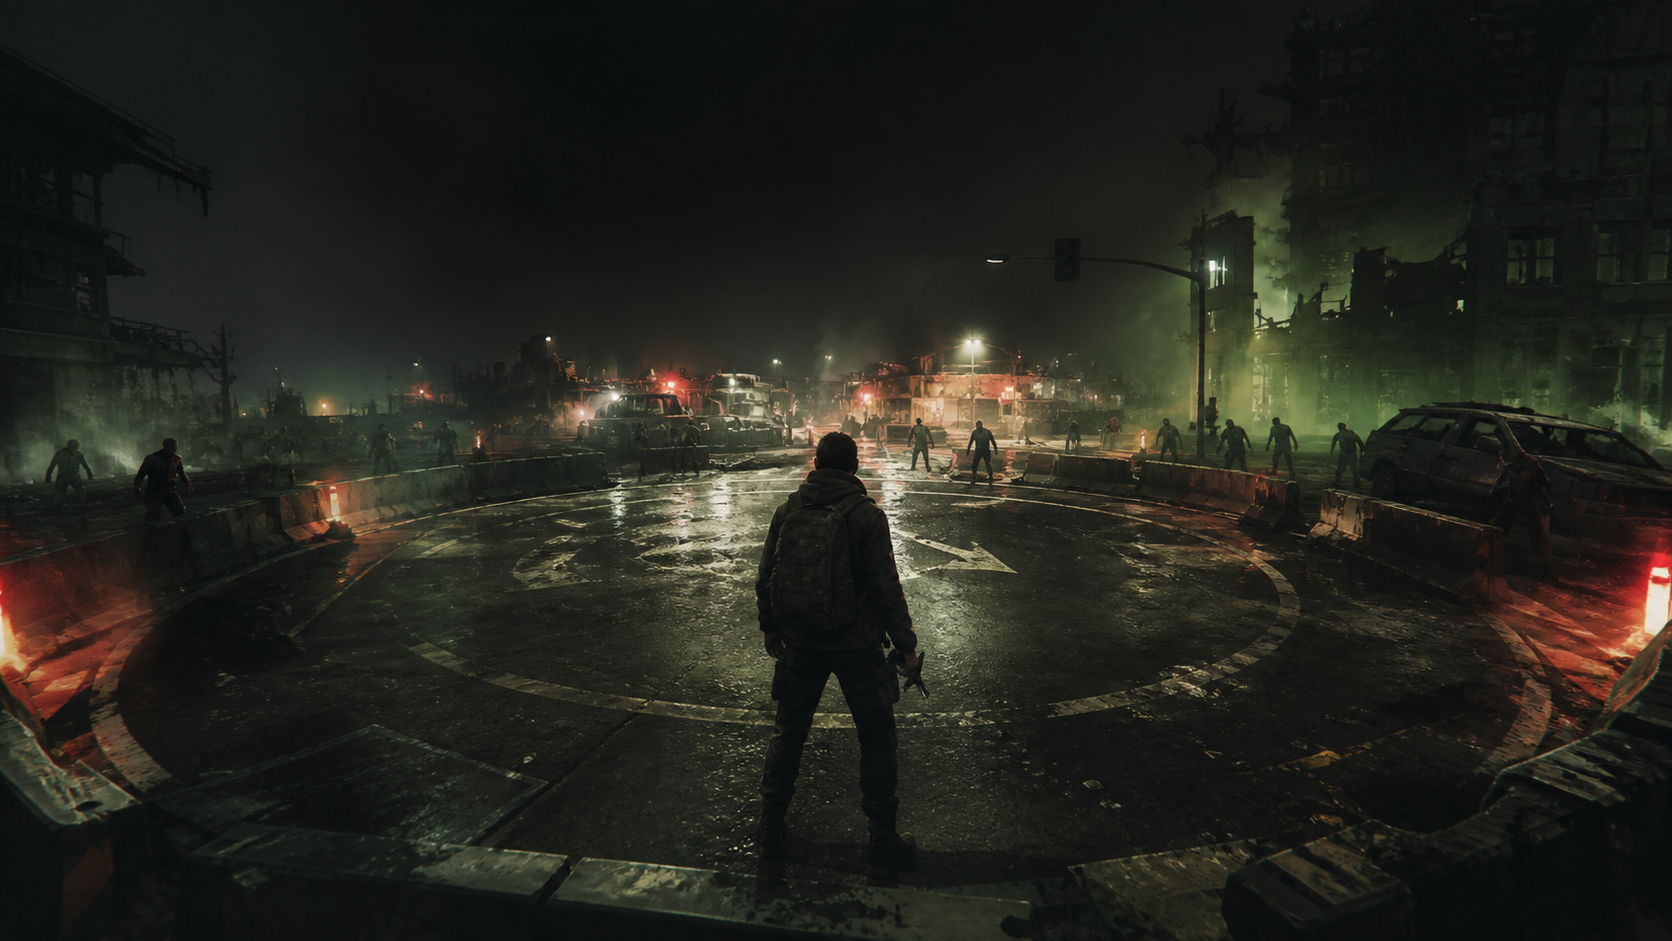
\includegraphics[width=0.88\textwidth]{outbreak-command-center.png}
\vfill
{\Large\bfseries Ficha técnica del repositorio\par}
\vspace{0.4cm}
Proyecto 1 de Modelación y Simulación --- Sección 30\par
Grupo 1 --- 2026\par
\vspace{0.45cm}
\href{https://github.com/DanielBarillasM/Proyecto-1_Grupo-1_Modelacion-y-Simulacion_Sec-30}%
{\color{green!35!white}\texttt{github.com/DanielBarillasM/Proyecto-1\_Grupo-1\_...}}
\end{titlepage}
\hypersetup{pageanchor=true}
\nopagecolor\color{ink}

\band{Propósito y alcance}

Se modela el subsistema real de aparición y balance de enemigos de un
videojuego. Los tiempos aleatorios alimentan movimiento y combate para estimar
la probabilidad de sobrevivir una misión de 90 segundos.

\textbf{Pregunta:} ¿cómo cambian congestión y supervivencia cuando se conserva
la media de los interarribos, pero cambia su distribución?

\begin{itemize}
  \item Poisson homogéneo con interarribos exponenciales por inversa.
  \item Renovación Polar--lognormal, positiva y con CV configurable.
  \item Marsaglia Polar frente a Box--Muller para la misma $N(0,1)$.
  \item Monte Carlo pareado, Wilson, McNemar, Wilcoxon y bootstrap.
\end{itemize}

\band{Modelo y escenario base}

\begin{tabularx}{\textwidth}{>{\bfseries}p{3.5cm}X X}
\toprule
Componente & Modelo & Propósito \\
\midrule
Llegada principal & $\Delta=-\ln(U)/\lambda$ & Poisson de tasa constante \\
Llegada alternativa & $\Delta=e^{\mu+\sigma Z}$ & Igual media, CV distinto \\
Combate & Paso $dt=0.05$ s & Movimiento, alcance, contacto y daño \\
Visualización & Plotly \texttt{Mesh3d} & Escena navegable en Streamlit \\
\bottomrule
\end{tabularx}

\begin{center}
\begin{tabular}{lrlrlr}
\toprule
Tasa & 55.8/min & CV Polar & 0.60 & Horizonte & 90 s \\
HP jugador & 110 & DPS jugador & 42 & Alcance & 10 m \\
HP infectado & 42 & Velocidad & 1.55 m/s & DPS & 9.5 \\
\bottomrule
\end{tabular}
\end{center}

La configuración evita la saturación cerca del 100\,\% y produce pares
discordantes informativos. Es una calibración de demostración, no telemetría.

\newpage
\band{Validación y comparación algorítmica}

La batería contiene \TestCount{} contrastes con corrección de Holm: PCG64,
LCG propio, transformaciones, independencia, aceptación y conteo Poisson. Un
contador uniforme pero predecible aprueba forma y falla las tres pruebas de
dependencia, por lo que actúa como control negativo.

\begin{figure}[H]
\centering
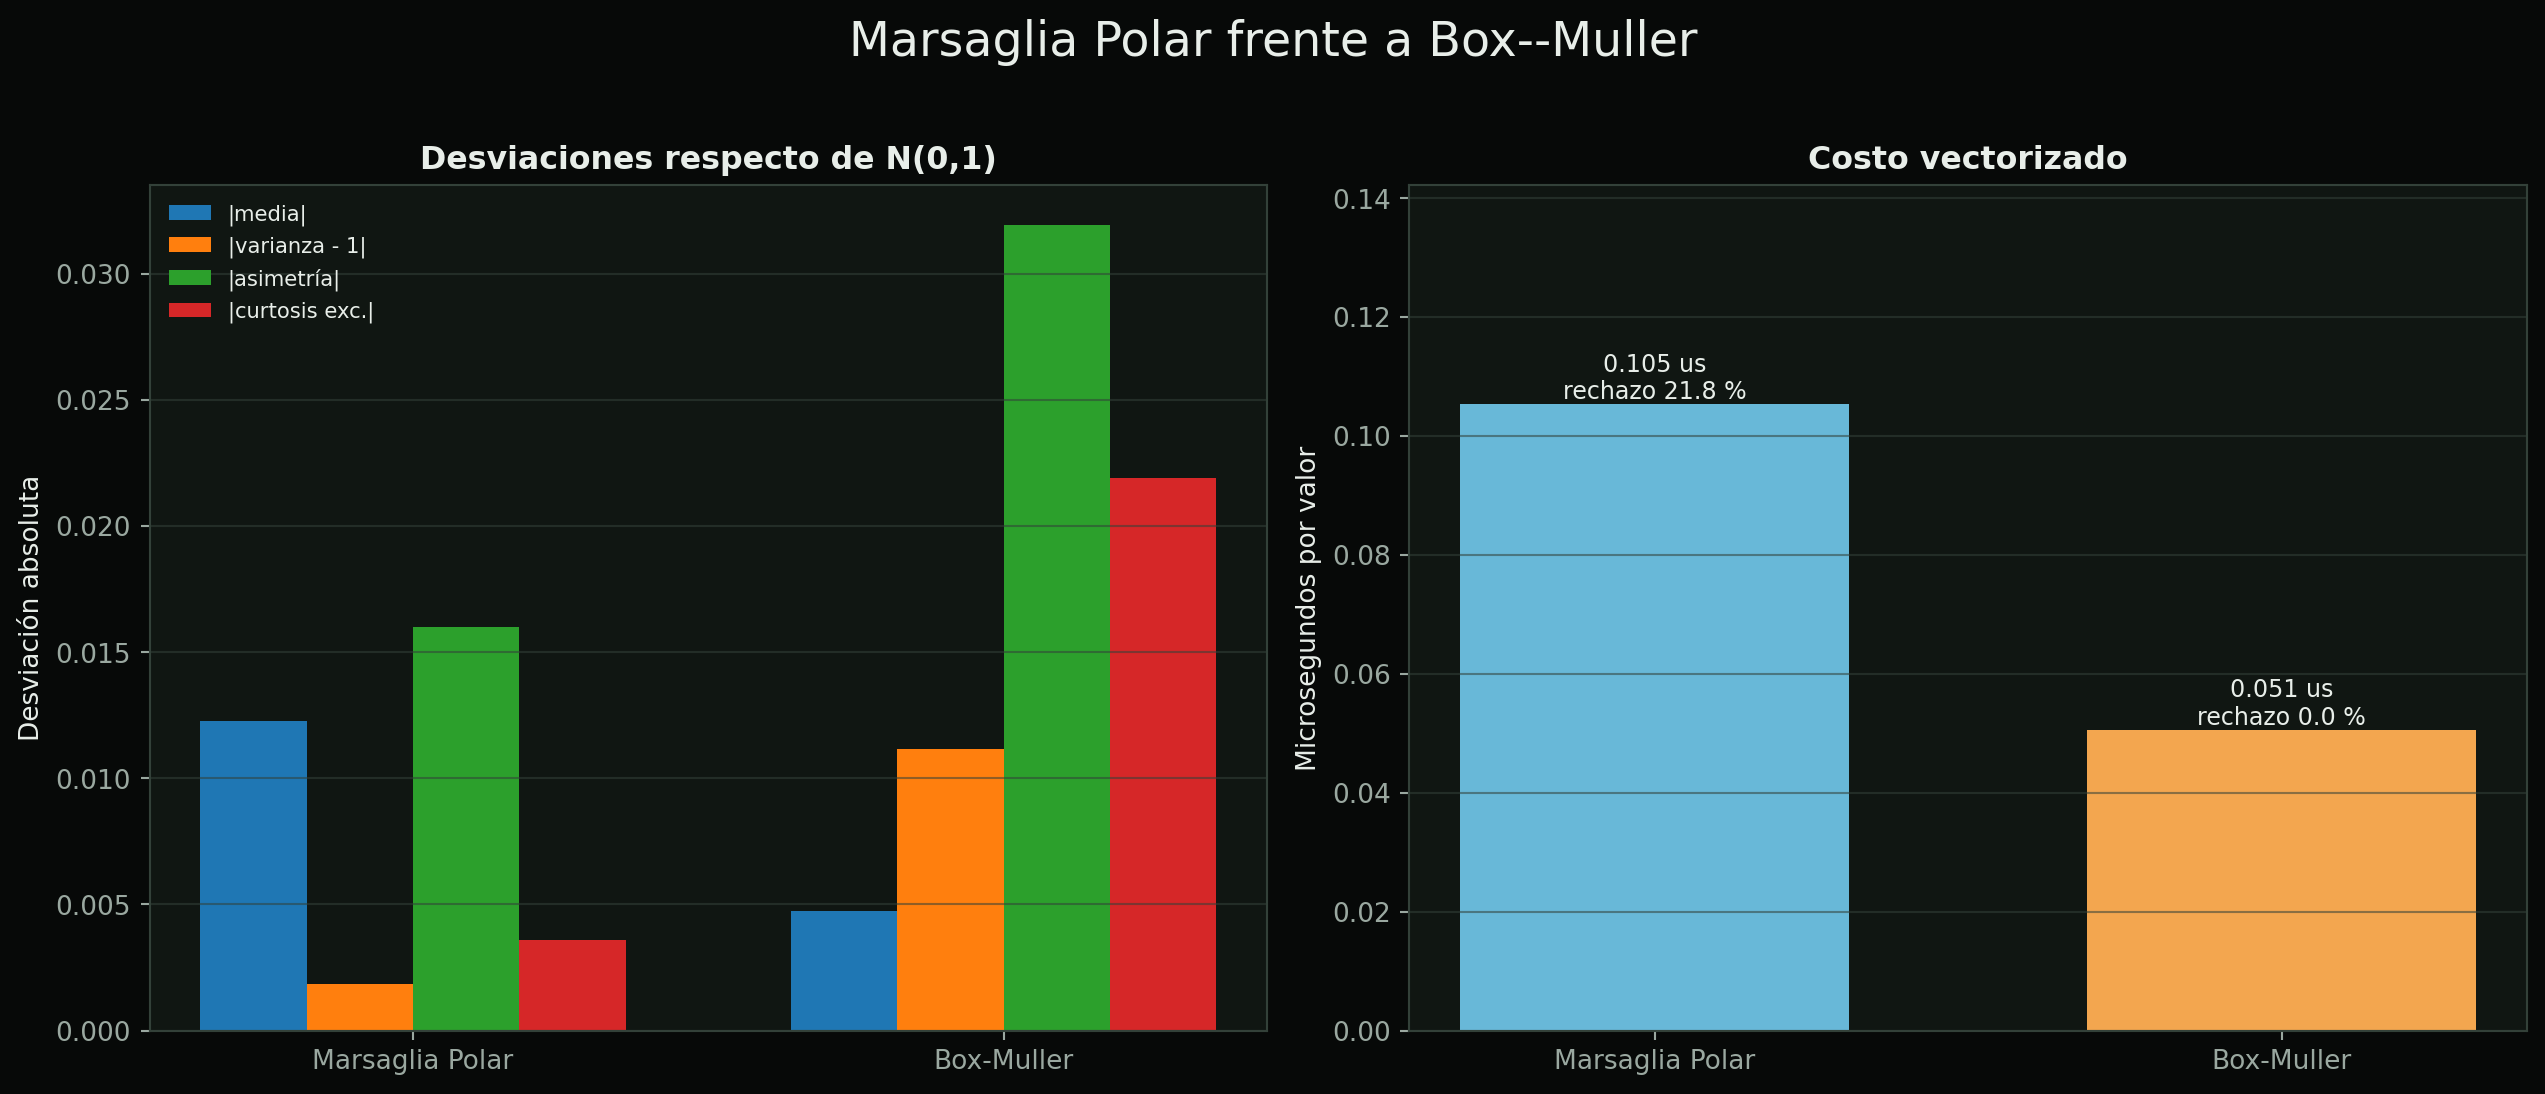
\includegraphics[width=0.96\textwidth]{report-normal-method-comparison.png}
\end{figure}

\begin{tabular}{lrrrr}
\toprule
Método & KS $p$ & $\mu$s/valor & Rechazo & Puntaje / 5 \\
\midrule
Marsaglia Polar & \PolarNormalKSP & \PolarNormalMicros & \PolarRejectedPercent\,\% & \PolarMethodScore \\
Box--Muller & \BoxMullerKSP & \BoxMullerMicros & 0\,\% & \BoxMullerMethodScore \\
\bottomrule
\end{tabular}

Ambos métodos son compatibles con $N(0,1)$. La matriz favorece a
\NormalMethodWinner{} en el equipo de referencia. Polar se conserva porque
materializa aceptación--rechazo; un valor $p$ mayor no se interpreta como mejor.

\band{Resultados de 400 corridas por modelo}

\begin{tabular}{lrr}
\toprule
Métrica & Poisson & Polar--lognormal \\
\midrule
Supervivencia & \PoissonSurvival\,\% & \PolarSurvival\,\% \\
IC Wilson 95\,\% & [\PoissonCILow, \PoissonCIHigh]\,\% & [\PolarCILow, \PolarCIHigh]\,\% \\
Tiempo medio & \PoissonMeanTime{} s & \PolarMeanTime{} s \\
Pico activo medio & \PoissonPeak & \PolarPeak \\
\bottomrule
\end{tabular}

Efecto Poisson menos Polar: \SurvivalDifference{} puntos porcentuales, IC
[\SurvivalDiffLow, \SurvivalDiffHigh] y McNemar $p=\McNemarP$. Es evidencia
para este escenario, no superioridad universal de una distribución.

\newpage
\band{Arquitectura y uso}

\begin{tabularx}{\textwidth}{>{\ttfamily}p{4.2cm}X}
\toprule
Ruta & Responsabilidad \\
\midrule
App/simulation.py & Motor, generadores, validación e inferencia \\
App/visuals.py & Gráficas Plotly y escena 3D \\
App/app.py & Interfaz, controles, estado y caché \\
report/ & Informe, CSV y figuras regenerables \\
presentation/ & HTML, ficha y guion dividido \\
tests/ & 28 pruebas automatizadas \\
\bottomrule
\end{tabularx}

\textbf{Inicio rápido}
\begin{verbatim}
cd zombie_poisson_streamlit
python -m venv .venv
python -m pip install -r requirements/requirements.txt
python -m streamlit run App/app.py
\end{verbatim}

\textbf{Entregables:} aplicación Streamlit, README, informe LaTeX/PDF, CSV,
presentación HTML offline, ficha DOCX/PDF y guion LaTeX/PDF dividido entre
Pablo Daniel Barillas Moreno, Jorge Palacios, Adrián Ricardo González Muralles,
Andrés Rafael Chivalán y Javier Andrés Chen.

\band{Límites y lectura responsable}

La tasa es constante; el jugador no se desplaza; los obstáculos son visuales;
el combate usa paso finito; no existe calibración con telemetría real. Los
valores $p$ no miden importancia práctica y los benchmarks dependen del equipo.

\textbf{Conclusión:} Poisson permanece como modelo principal por parsimonia,
interpretación y correspondencia exacta entre conteo e interarribos. La
alternativa demuestra que igual media no implica iguales rachas, concurrencia
o supervivencia; la comparación Box--Muller separa esa conclusión de la
eficiencia del algoritmo que produce normales.

\end{document}
